\documentclass[twoside]{book}

% Packages required by doxygen
\usepackage{fixltx2e}
\usepackage{calc}
\usepackage{doxygen}
\usepackage[export]{adjustbox} % also loads graphicx
\usepackage{graphicx}
\usepackage[utf8]{inputenc}
\usepackage{makeidx}
\usepackage{multicol}
\usepackage{multirow}
\PassOptionsToPackage{warn}{textcomp}
\usepackage{textcomp}
\usepackage[nointegrals]{wasysym}
\usepackage[table]{xcolor}

% Font selection
\usepackage[T1]{fontenc}
\usepackage[scaled=.90]{helvet}
\usepackage{courier}
\usepackage{amssymb}
\usepackage{sectsty}
\renewcommand{\familydefault}{\sfdefault}
\allsectionsfont{%
  \fontseries{bc}\selectfont%
  \color{darkgray}%
}
\renewcommand{\DoxyLabelFont}{%
  \fontseries{bc}\selectfont%
  \color{darkgray}%
}
\newcommand{\+}{\discretionary{\mbox{\scriptsize$\hookleftarrow$}}{}{}}

% Page & text layout
\usepackage{geometry}
\geometry{%
  a4paper,%
  top=2.5cm,%
  bottom=2.5cm,%
  left=2.5cm,%
  right=2.5cm%
}
\tolerance=750
\hfuzz=15pt
\hbadness=750
\setlength{\emergencystretch}{15pt}
\setlength{\parindent}{0cm}
\setlength{\parskip}{3ex plus 2ex minus 2ex}
\makeatletter
\renewcommand{\paragraph}{%
  \@startsection{paragraph}{4}{0ex}{-1.0ex}{1.0ex}{%
    \normalfont\normalsize\bfseries\SS@parafont%
  }%
}
\renewcommand{\subparagraph}{%
  \@startsection{subparagraph}{5}{0ex}{-1.0ex}{1.0ex}{%
    \normalfont\normalsize\bfseries\SS@subparafont%
  }%
}
\makeatother

% Headers & footers
\usepackage{fancyhdr}
\pagestyle{fancyplain}
\fancyhead[LE]{\fancyplain{}{\bfseries\thepage}}
\fancyhead[CE]{\fancyplain{}{}}
\fancyhead[RE]{\fancyplain{}{\bfseries\leftmark}}
\fancyhead[LO]{\fancyplain{}{\bfseries\rightmark}}
\fancyhead[CO]{\fancyplain{}{}}
\fancyhead[RO]{\fancyplain{}{\bfseries\thepage}}
\fancyfoot[LE]{\fancyplain{}{}}
\fancyfoot[CE]{\fancyplain{}{}}
\fancyfoot[RE]{\fancyplain{}{\bfseries\scriptsize Generated by Doxygen }}
\fancyfoot[LO]{\fancyplain{}{\bfseries\scriptsize Generated by Doxygen }}
\fancyfoot[CO]{\fancyplain{}{}}
\fancyfoot[RO]{\fancyplain{}{}}
\renewcommand{\footrulewidth}{0.4pt}
\renewcommand{\chaptermark}[1]{%
  \markboth{#1}{}%
}
\renewcommand{\sectionmark}[1]{%
  \markright{\thesection\ #1}%
}

% Indices & bibliography
\usepackage{natbib}
\usepackage[titles]{tocloft}
\setcounter{tocdepth}{3}
\setcounter{secnumdepth}{5}
\makeindex

% Hyperlinks (required, but should be loaded last)
\usepackage{ifpdf}
\ifpdf
  \usepackage[pdftex,pagebackref=true]{hyperref}
\else
  \usepackage[ps2pdf,pagebackref=true]{hyperref}
\fi
\hypersetup{%
  colorlinks=true,%
  linkcolor=blue,%
  citecolor=blue,%
  unicode%
}

% Custom commands
\newcommand{\clearemptydoublepage}{%
  \newpage{\pagestyle{empty}\cleardoublepage}%
}

\usepackage{caption}
\captionsetup{labelsep=space,justification=centering,font={bf},singlelinecheck=off,skip=4pt,position=top}

%===== C O N T E N T S =====

\begin{document}

% Titlepage & ToC
\hypersetup{pageanchor=false,
             bookmarksnumbered=true,
             pdfencoding=unicode
            }
\pagenumbering{roman}
\begin{titlepage}
\vspace*{7cm}
\begin{center}%
{\Large My Project }\\
\vspace*{1cm}
{\large Generated by Doxygen 1.8.11}\\
\end{center}
\end{titlepage}
\clearemptydoublepage
\tableofcontents
\clearemptydoublepage
\pagenumbering{arabic}
\hypersetup{pageanchor=true}

%--- Begin generated contents ---
\chapter{Class Index}
\section{Class List}
Here are the classes, structs, unions and interfaces with brief descriptions\+:\begin{DoxyCompactList}
\item\contentsline{section}{\hyperlink{unionsemun}{semun} }{\pageref{unionsemun}}{}
\end{DoxyCompactList}

\chapter{File Index}
\section{File List}
Here is a list of all documented files with brief descriptions\+:\begin{DoxyCompactList}
\item\contentsline{section}{\hyperlink{Ejercicio2_8c}{Ejercicio2.\+c} \\*Ejercicio 2 de la Practica 2 }{\pageref{Ejercicio2_8c}}{}
\item\contentsline{section}{\hyperlink{Ejercicio4_8c}{Ejercicio4.\+c} \\*Ejercicio 4 de la Practica 2 }{\pageref{Ejercicio4_8c}}{}
\item\contentsline{section}{\hyperlink{Ejercicio6a_8c}{Ejercicio6a.\+c} \\*Ejercicio 6a de la Practica 2 }{\pageref{Ejercicio6a_8c}}{}
\item\contentsline{section}{\hyperlink{Ejercicio6b_8c}{Ejercicio6b.\+c} \\*Ejercicio 6b de la Practica 2 }{\pageref{Ejercicio6b_8c}}{}
\item\contentsline{section}{\hyperlink{Ejercicio8_8c}{Ejercicio8.\+c} \\*Ejercicio 8 de la Practica 2 }{\pageref{Ejercicio8_8c}}{}
\item\contentsline{section}{\hyperlink{Ejercicio8_8h}{Ejercicio8.\+h} \\*Ejercicio 8 de la Practica 2 }{\pageref{Ejercicio8_8h}}{}
\item\contentsline{section}{\hyperlink{Ejercicio9_8c}{Ejercicio9.\+c} \\*Ejercicio 9 de la Practica 2 }{\pageref{Ejercicio9_8c}}{}
\end{DoxyCompactList}

\chapter{Class Documentation}
\hypertarget{struct__message}{}\section{\+\_\+message Struct Reference}
\label{struct__message}\index{\+\_\+message@{\+\_\+message}}
\subsection*{Public Attributes}
\begin{DoxyCompactItemize}
\item 
long {\bfseries type}\hypertarget{struct__message_a0ed689031575cf4ef7330f807cfd8c2f}{}\label{struct__message_a0ed689031575cf4ef7330f807cfd8c2f}

\item 
char {\bfseries text} \mbox{[}16\mbox{]}\hypertarget{struct__message_a390dbde354d571c3d1fbcffda32798d2}{}\label{struct__message_a390dbde354d571c3d1fbcffda32798d2}

\item 
int {\bfseries flag}\hypertarget{struct__message_a6ab433a62c87c70cf3af3900449df656}{}\label{struct__message_a6ab433a62c87c70cf3af3900449df656}

\end{DoxyCompactItemize}


The documentation for this struct was generated from the following file\+:\begin{DoxyCompactItemize}
\item 
\hyperlink{Ejercicio5_8c}{Ejercicio5.\+c}\end{DoxyCompactItemize}

\hypertarget{structinfo}{}\section{info Struct Reference}
\label{structinfo}\index{info@{info}}
\subsection*{Public Attributes}
\begin{DoxyCompactItemize}
\item 
char {\bfseries nombre} \mbox{[}80\mbox{]}\hypertarget{structinfo_a0de2dc94039ebaa93065006cf9cbb172}{}\label{structinfo_a0de2dc94039ebaa93065006cf9cbb172}

\item 
int {\bfseries id}\hypertarget{structinfo_afe86f23d8bd5fd8d139e39a5b1a01171}{}\label{structinfo_afe86f23d8bd5fd8d139e39a5b1a01171}

\item 
char {\bfseries array} \mbox{[}N\mbox{]}\hypertarget{structinfo_a0a0a04bfaa64287b11d085e6f859a4ad}{}\label{structinfo_a0a0a04bfaa64287b11d085e6f859a4ad}

\item 
int {\bfseries contador}\hypertarget{structinfo_afb848f971a0f63b924dc83681e8930c5}{}\label{structinfo_afb848f971a0f63b924dc83681e8930c5}

\end{DoxyCompactItemize}


The documentation for this struct was generated from the following files\+:\begin{DoxyCompactItemize}
\item 
\hyperlink{Ejercicio2_8c}{Ejercicio2.\+c}\item 
\hyperlink{Ejercicio2__solved_8c}{Ejercicio2\+\_\+solved.\+c}\item 
\hyperlink{Ejercicio3_8c}{Ejercicio3.\+c}\end{DoxyCompactItemize}

\hypertarget{unionsemun}{}\section{semun Union Reference}
\label{unionsemun}\index{semun@{semun}}
\subsection*{Public Attributes}
\begin{DoxyCompactItemize}
\item 
int {\bfseries val}\hypertarget{unionsemun_ac6121ecb6d04a024e07e12bd71b94031}{}\label{unionsemun_ac6121ecb6d04a024e07e12bd71b94031}

\item 
struct semid\+\_\+ds $\ast$ {\bfseries semstat}\hypertarget{unionsemun_afb976847aea44952be2118ad0329d832}{}\label{unionsemun_afb976847aea44952be2118ad0329d832}

\item 
unsigned short $\ast$ {\bfseries array}\hypertarget{unionsemun_aca23b8e730a0553205813c0cb7692b54}{}\label{unionsemun_aca23b8e730a0553205813c0cb7692b54}

\end{DoxyCompactItemize}


The documentation for this union was generated from the following file\+:\begin{DoxyCompactItemize}
\item 
\hyperlink{Ejercicio8_8c}{Ejercicio8.\+c}\end{DoxyCompactItemize}

\chapter{File Documentation}
\hypertarget{Ejercicio2_8c}{}\section{Ejercicio2.\+c File Reference}
\label{Ejercicio2_8c}\index{Ejercicio2.\+c@{Ejercicio2.\+c}}


Primera parte del ejercicio 2 de la Practica 3.  


{\ttfamily \#include $<$stdio.\+h$>$}\\*
{\ttfamily \#include $<$string.\+h$>$}\\*
{\ttfamily \#include $<$sys/types.\+h$>$}\\*
{\ttfamily \#include $<$sys/wait.\+h$>$}\\*
{\ttfamily \#include $<$stdlib.\+h$>$}\\*
{\ttfamily \#include $<$unistd.\+h$>$}\\*
{\ttfamily \#include $<$signal.\+h$>$}\\*
{\ttfamily \#include $<$sys/shm.\+h$>$}\\*
{\ttfamily \#include $<$errno.\+h$>$}\\*
Include dependency graph for Ejercicio2.\+c\+:

\hypertarget{Ejercicio2__solved_8c}{}\section{Ejercicio2\+\_\+solved.\+c File Reference}
\label{Ejercicio2__solved_8c}\index{Ejercicio2\+\_\+solved.\+c@{Ejercicio2\+\_\+solved.\+c}}


Segunda parte del ejercicio 2 de la Practica 3.  


{\ttfamily \#include $<$stdio.\+h$>$}\\*
{\ttfamily \#include $<$string.\+h$>$}\\*
{\ttfamily \#include $<$sys/types.\+h$>$}\\*
{\ttfamily \#include $<$sys/wait.\+h$>$}\\*
{\ttfamily \#include $<$stdlib.\+h$>$}\\*
{\ttfamily \#include $<$unistd.\+h$>$}\\*
{\ttfamily \#include $<$signal.\+h$>$}\\*
{\ttfamily \#include $<$sys/shm.\+h$>$}\\*
{\ttfamily \#include $<$errno.\+h$>$}\\*
{\ttfamily \#include \char`\"{}Libreria\+Semaforos.\+h\char`\"{}}\\*
Include dependency graph for Ejercicio2\+\_\+solved.\+c\+:
% FIG 0
\subsection*{Classes}
\begin{DoxyCompactItemize}
\item 
struct \hyperlink{structinfo}{info}
\end{DoxyCompactItemize}
\subsection*{Macros}
\begin{DoxyCompactItemize}
\item 
\#define {\bfseries S\+E\+M\+K\+EY}~75798\hypertarget{Ejercicio2__solved_8c_ada831b9e37399bf906c8184a888e28cd}{}\label{Ejercicio2__solved_8c_ada831b9e37399bf906c8184a888e28cd}

\item 
\#define {\bfseries N\+\_\+\+S\+E\+M\+A\+F\+O\+R\+OS}~1\hypertarget{Ejercicio2__solved_8c_a95c81905ff3d55e62fb763f407f9fab1}{}\label{Ejercicio2__solved_8c_a95c81905ff3d55e62fb763f407f9fab1}

\item 
\#define {\bfseries F\+I\+L\+E\+K\+EY}~\char`\"{}/bin/cat\char`\"{}\hypertarget{Ejercicio2__solved_8c_a68c15c5fb7f7c6f707903e6a46ab0557}{}\label{Ejercicio2__solved_8c_a68c15c5fb7f7c6f707903e6a46ab0557}

\item 
\#define {\bfseries K\+EY}~1300\hypertarget{Ejercicio2__solved_8c_a8ae9d53f33f46cfcfcb9736e6351452a}{}\label{Ejercicio2__solved_8c_a8ae9d53f33f46cfcfcb9736e6351452a}

\item 
\#define \hyperlink{Ejercicio2__solved_8c_a9dd395f2e0046c1513c84dfcfb9e54da}{N\+U\+M\+\_\+\+H\+I\+J\+OS}~5
\end{DoxyCompactItemize}
\subsection*{Typedefs}
\begin{DoxyCompactItemize}
\item 
typedef struct \hyperlink{structinfo}{info} {\bfseries Info}\hypertarget{Ejercicio2__solved_8c_a163511f3dadd6f89b69b2c2b6d40dcf7}{}\label{Ejercicio2__solved_8c_a163511f3dadd6f89b69b2c2b6d40dcf7}

\end{DoxyCompactItemize}
\subsection*{Functions}
\begin{DoxyCompactItemize}
\item 
int \hyperlink{Ejercicio2__solved_8c_a423be02d237888f767b6d107096c10f4}{aleat\+\_\+num} (int inf, int sup)
\begin{DoxyCompactList}\small\item\em Funcion a la que le pasas 2 numeros y devuelve un numero aleatorio entre ambos. \end{DoxyCompactList}\item 
void \hyperlink{Ejercicio2__solved_8c_a0897883a0dfdf1023f377e262cee1299}{captura} ()\hypertarget{Ejercicio2__solved_8c_a0897883a0dfdf1023f377e262cee1299}{}\label{Ejercicio2__solved_8c_a0897883a0dfdf1023f377e262cee1299}

\begin{DoxyCompactList}\small\item\em Funcion que ejecuta el proceso padre tras recibir la senal S\+I\+G\+U\+S\+R1. En esta funcion se lee la region de zona compartida y se imprime el nombre del usuario y su id. En este caso para solucionar el problema de que varios procesos accedan a la memoria compartida a la vez, se realiza un down de un semaforo justo antes de acceder a la memoria compartida y un up al acabar de acceder a esta. \end{DoxyCompactList}\item 
int \hyperlink{Ejercicio2__solved_8c_ae66f6b31b5ad750f1fe042a706a4e3d4}{main} ()
\begin{DoxyCompactList}\small\item\em El proceso padre crea N hijos cada uno de los cuales primero duerme un tiempo aleatorio entre 1 y 5 segundos y luego pide por pantalla el nombre de un nuevo usuario y pone este usuario en la memoria compartida aumentando en 1 el id para que este no se repita en 2 usuarios. Tras añadir un usuario los procesos hijo mandan la señal S\+I\+G\+U\+S\+R1 al padre para que este ejecute la funcion de control de esta senal que imprime por pantalla el nombre y el id del usuario que esta en la memoria compartida. Para la sincronizacion en este caso, para evitar que varios procesos entren a la vez a la memoria compartida se realiza mediante semaforos haciendo un down antes de acceder a esta y un up al terminar de acceder. \end{DoxyCompactList}\end{DoxyCompactItemize}
\subsection*{Variables}
\begin{DoxyCompactItemize}
\item 
int {\bfseries semid}\hypertarget{Ejercicio2__solved_8c_a7c35ac5305085cf7360645b8d52988b5}{}\label{Ejercicio2__solved_8c_a7c35ac5305085cf7360645b8d52988b5}

\item 
int {\bfseries id\+\_\+zone}\hypertarget{Ejercicio2__solved_8c_a554bdf03ae4f8480bddb761bd7c03b53}{}\label{Ejercicio2__solved_8c_a554bdf03ae4f8480bddb761bd7c03b53}

\end{DoxyCompactItemize}


\subsection{Detailed Description}
Segunda parte del ejercicio 2 de la Practica 3. 

\begin{DoxyAuthor}{Author}
\href{mailto:Javier.delgadod@estudiante.uam.es}{\tt Javier.\+delgadod@estudiante.\+uam.\+es} 

\href{mailto:Javier.lopezcano@estudiante.uam.es}{\tt Javier.\+lopezcano@estudiante.\+uam.\+es} 
\end{DoxyAuthor}


\subsection{Macro Definition Documentation}
\index{Ejercicio2\+\_\+solved.\+c@{Ejercicio2\+\_\+solved.\+c}!N\+U\+M\+\_\+\+H\+I\+J\+OS@{N\+U\+M\+\_\+\+H\+I\+J\+OS}}
\index{N\+U\+M\+\_\+\+H\+I\+J\+OS@{N\+U\+M\+\_\+\+H\+I\+J\+OS}!Ejercicio2\+\_\+solved.\+c@{Ejercicio2\+\_\+solved.\+c}}
\subsubsection[{\texorpdfstring{N\+U\+M\+\_\+\+H\+I\+J\+OS}{NUM_HIJOS}}]{\setlength{\rightskip}{0pt plus 5cm}\#define N\+U\+M\+\_\+\+H\+I\+J\+OS~5}\hypertarget{Ejercicio2__solved_8c_a9dd395f2e0046c1513c84dfcfb9e54da}{}\label{Ejercicio2__solved_8c_a9dd395f2e0046c1513c84dfcfb9e54da}
Numero de hijos que crea el proceso padre 

\subsection{Function Documentation}
\index{Ejercicio2\+\_\+solved.\+c@{Ejercicio2\+\_\+solved.\+c}!aleat\+\_\+num@{aleat\+\_\+num}}
\index{aleat\+\_\+num@{aleat\+\_\+num}!Ejercicio2\+\_\+solved.\+c@{Ejercicio2\+\_\+solved.\+c}}
\subsubsection[{\texorpdfstring{aleat\+\_\+num(int inf, int sup)}{aleat_num(int inf, int sup)}}]{\setlength{\rightskip}{0pt plus 5cm}int aleat\+\_\+num (
\begin{DoxyParamCaption}
\item[{int}]{inf, }
\item[{int}]{sup}
\end{DoxyParamCaption}
)}\hypertarget{Ejercicio2__solved_8c_a423be02d237888f767b6d107096c10f4}{}\label{Ejercicio2__solved_8c_a423be02d237888f767b6d107096c10f4}


Funcion a la que le pasas 2 numeros y devuelve un numero aleatorio entre ambos. 


\begin{DoxyParams}{Parameters}
{\em inf} & Int con el numero mas bajo que se quiere. \\
\hline
{\em sup} & Int con el numero mas alto que se quiere. \\
\hline
\end{DoxyParams}
\begin{DoxyReturn}{Returns}
int con un número aleatorio entre inf y sup. 
\end{DoxyReturn}
\index{Ejercicio2\+\_\+solved.\+c@{Ejercicio2\+\_\+solved.\+c}!main@{main}}
\index{main@{main}!Ejercicio2\+\_\+solved.\+c@{Ejercicio2\+\_\+solved.\+c}}
\subsubsection[{\texorpdfstring{main()}{main()}}]{\setlength{\rightskip}{0pt plus 5cm}int main (
\begin{DoxyParamCaption}
{}
\end{DoxyParamCaption}
)}\hypertarget{Ejercicio2__solved_8c_ae66f6b31b5ad750f1fe042a706a4e3d4}{}\label{Ejercicio2__solved_8c_ae66f6b31b5ad750f1fe042a706a4e3d4}


El proceso padre crea N hijos cada uno de los cuales primero duerme un tiempo aleatorio entre 1 y 5 segundos y luego pide por pantalla el nombre de un nuevo usuario y pone este usuario en la memoria compartida aumentando en 1 el id para que este no se repita en 2 usuarios. Tras añadir un usuario los procesos hijo mandan la señal S\+I\+G\+U\+S\+R1 al padre para que este ejecute la funcion de control de esta senal que imprime por pantalla el nombre y el id del usuario que esta en la memoria compartida. Para la sincronizacion en este caso, para evitar que varios procesos entren a la vez a la memoria compartida se realiza mediante semaforos haciendo un down antes de acceder a esta y un up al terminar de acceder. 

\begin{DoxyReturn}{Returns}
int que determina si el programa se ha ejecutado o no con exito. 
\end{DoxyReturn}

\hypertarget{Ejercicio3_8c}{}\section{Ejercicio3.\+c File Reference}
\label{Ejercicio3_8c}\index{Ejercicio3.\+c@{Ejercicio3.\+c}}


Ejercicio 3 de la Practica 3.  


{\ttfamily \#include $<$stdio.\+h$>$}\\*
{\ttfamily \#include $<$string.\+h$>$}\\*
{\ttfamily \#include $<$sys/types.\+h$>$}\\*
{\ttfamily \#include $<$sys/wait.\+h$>$}\\*
{\ttfamily \#include $<$stdlib.\+h$>$}\\*
{\ttfamily \#include $<$unistd.\+h$>$}\\*
{\ttfamily \#include $<$signal.\+h$>$}\\*
{\ttfamily \#include $<$sys/shm.\+h$>$}\\*
{\ttfamily \#include $<$errno.\+h$>$}\\*
{\ttfamily \#include \char`\"{}Libreria\+Semaforos.\+h\char`\"{}}\\*
Include dependency graph for Ejercicio3.\+c\+:
% FIG 0
\subsection*{Classes}
\begin{DoxyCompactItemize}
\item 
struct \hyperlink{structinfo}{info}
\end{DoxyCompactItemize}
\subsection*{Macros}
\begin{DoxyCompactItemize}
\item 
\#define {\bfseries S\+E\+M\+K\+EY}~75798\hypertarget{Ejercicio3_8c_ada831b9e37399bf906c8184a888e28cd}{}\label{Ejercicio3_8c_ada831b9e37399bf906c8184a888e28cd}

\item 
\#define {\bfseries N\+\_\+\+S\+E\+M\+A\+F\+O\+R\+OS}~1\hypertarget{Ejercicio3_8c_a95c81905ff3d55e62fb763f407f9fab1}{}\label{Ejercicio3_8c_a95c81905ff3d55e62fb763f407f9fab1}

\item 
\#define {\bfseries F\+I\+L\+E\+K\+EY}~\char`\"{}/bin/cat\char`\"{}\hypertarget{Ejercicio3_8c_a68c15c5fb7f7c6f707903e6a46ab0557}{}\label{Ejercicio3_8c_a68c15c5fb7f7c6f707903e6a46ab0557}

\item 
\#define {\bfseries K\+EY}~1300\hypertarget{Ejercicio3_8c_a8ae9d53f33f46cfcfcb9736e6351452a}{}\label{Ejercicio3_8c_a8ae9d53f33f46cfcfcb9736e6351452a}

\item 
\#define {\bfseries N}~36\hypertarget{Ejercicio3_8c_a0240ac851181b84ac374872dc5434ee4}{}\label{Ejercicio3_8c_a0240ac851181b84ac374872dc5434ee4}

\end{DoxyCompactItemize}
\subsection*{Typedefs}
\begin{DoxyCompactItemize}
\item 
typedef struct \hyperlink{structinfo}{info} {\bfseries Info}\hypertarget{Ejercicio3_8c_a163511f3dadd6f89b69b2c2b6d40dcf7}{}\label{Ejercicio3_8c_a163511f3dadd6f89b69b2c2b6d40dcf7}

\end{DoxyCompactItemize}
\subsection*{Functions}
\begin{DoxyCompactItemize}
\item 
int \hyperlink{Ejercicio3_8c_af6be62fb8af1ca164fa2861c403b8245}{produce\+\_\+item} ()
\begin{DoxyCompactList}\small\item\em Funcion que produce los elementos, que en este caso son caracteres. crea los caracteres de la \textquotesingle{}a\textquotesingle{} a la \textquotesingle{}z\textquotesingle{} y los numeros del 0 al 9 y los almacena en la memoria compartida. \end{DoxyCompactList}\item 
int \hyperlink{Ejercicio3_8c_a8a453d70ebc614f358646af9dcf7cd49}{consume\+\_\+item} ()
\begin{DoxyCompactList}\small\item\em Funcion que consume los elementos. En este caso consumirlos consiste en ir leyendolos de la memoria compartida e irlos imprimiendo por pantalla. \end{DoxyCompactList}\item 
int \hyperlink{Ejercicio3_8c_ae66f6b31b5ad750f1fe042a706a4e3d4}{main} ()
\begin{DoxyCompactList}\small\item\em El proceso padre inicializa una zona de memoria compartida y un semaforo paracontrolar el acceso a esta, tras esto crea un proceso hijo, que consume los elementos creados por el productor con la funcion \hyperlink{Ejercicio3_8c_a8a453d70ebc614f358646af9dcf7cd49}{consume\+\_\+item()} hasta que esta devuelve 0 en cuyo caso termina su ejecucion (pues se habra llegado ya al ultimo). Mientras tanto el padre se va encargando de producir los objetos e introducirlos en la memoria compartida con la funcion produce\+\_\+item, hasta que esta devuelve 0 indicando que se ha creado ya el ultimo elemento, tras lo cual espera a que acabe la ejecucion del hijo, libera la memoria compartida y los semaforos y termina su ejecucion. \end{DoxyCompactList}\end{DoxyCompactItemize}
\subsection*{Variables}
\begin{DoxyCompactItemize}
\item 
int {\bfseries semid}\hypertarget{Ejercicio3_8c_a7c35ac5305085cf7360645b8d52988b5}{}\label{Ejercicio3_8c_a7c35ac5305085cf7360645b8d52988b5}

\item 
int {\bfseries id\+\_\+zone}\hypertarget{Ejercicio3_8c_a554bdf03ae4f8480bddb761bd7c03b53}{}\label{Ejercicio3_8c_a554bdf03ae4f8480bddb761bd7c03b53}

\end{DoxyCompactItemize}


\subsection{Detailed Description}
Ejercicio 3 de la Practica 3. 

\begin{DoxyAuthor}{Author}
\href{mailto:Javier.delgadod@estudiante.uam.es}{\tt Javier.\+delgadod@estudiante.\+uam.\+es} 

\href{mailto:Javier.lopezcano@estudiante.uam.es}{\tt Javier.\+lopezcano@estudiante.\+uam.\+es} 
\end{DoxyAuthor}


\subsection{Function Documentation}
\index{Ejercicio3.\+c@{Ejercicio3.\+c}!consume\+\_\+item@{consume\+\_\+item}}
\index{consume\+\_\+item@{consume\+\_\+item}!Ejercicio3.\+c@{Ejercicio3.\+c}}
\subsubsection[{\texorpdfstring{consume\+\_\+item()}{consume_item()}}]{\setlength{\rightskip}{0pt plus 5cm}int consume\+\_\+item (
\begin{DoxyParamCaption}
{}
\end{DoxyParamCaption}
)}\hypertarget{Ejercicio3_8c_a8a453d70ebc614f358646af9dcf7cd49}{}\label{Ejercicio3_8c_a8a453d70ebc614f358646af9dcf7cd49}


Funcion que consume los elementos. En este caso consumirlos consiste en ir leyendolos de la memoria compartida e irlos imprimiendo por pantalla. 

\begin{DoxyReturn}{Returns}
int que indica si la funcion se ha ejecutado con exito. 
\end{DoxyReturn}
\index{Ejercicio3.\+c@{Ejercicio3.\+c}!main@{main}}
\index{main@{main}!Ejercicio3.\+c@{Ejercicio3.\+c}}
\subsubsection[{\texorpdfstring{main()}{main()}}]{\setlength{\rightskip}{0pt plus 5cm}int main (
\begin{DoxyParamCaption}
{}
\end{DoxyParamCaption}
)}\hypertarget{Ejercicio3_8c_ae66f6b31b5ad750f1fe042a706a4e3d4}{}\label{Ejercicio3_8c_ae66f6b31b5ad750f1fe042a706a4e3d4}


El proceso padre inicializa una zona de memoria compartida y un semaforo paracontrolar el acceso a esta, tras esto crea un proceso hijo, que consume los elementos creados por el productor con la funcion \hyperlink{Ejercicio3_8c_a8a453d70ebc614f358646af9dcf7cd49}{consume\+\_\+item()} hasta que esta devuelve 0 en cuyo caso termina su ejecucion (pues se habra llegado ya al ultimo). Mientras tanto el padre se va encargando de producir los objetos e introducirlos en la memoria compartida con la funcion produce\+\_\+item, hasta que esta devuelve 0 indicando que se ha creado ya el ultimo elemento, tras lo cual espera a que acabe la ejecucion del hijo, libera la memoria compartida y los semaforos y termina su ejecucion. 

\begin{DoxyReturn}{Returns}
int que determina si el programa se ha ejecutado o no con exito. 
\end{DoxyReturn}
\index{Ejercicio3.\+c@{Ejercicio3.\+c}!produce\+\_\+item@{produce\+\_\+item}}
\index{produce\+\_\+item@{produce\+\_\+item}!Ejercicio3.\+c@{Ejercicio3.\+c}}
\subsubsection[{\texorpdfstring{produce\+\_\+item()}{produce_item()}}]{\setlength{\rightskip}{0pt plus 5cm}int produce\+\_\+item (
\begin{DoxyParamCaption}
{}
\end{DoxyParamCaption}
)}\hypertarget{Ejercicio3_8c_af6be62fb8af1ca164fa2861c403b8245}{}\label{Ejercicio3_8c_af6be62fb8af1ca164fa2861c403b8245}


Funcion que produce los elementos, que en este caso son caracteres. crea los caracteres de la \textquotesingle{}a\textquotesingle{} a la \textquotesingle{}z\textquotesingle{} y los numeros del 0 al 9 y los almacena en la memoria compartida. 

\begin{DoxyReturn}{Returns}
int que indica si la funcion se ha ejecutado correctamente. 
\end{DoxyReturn}

\hypertarget{Ejercicio4_8c}{}\section{Ejercicio4.\+c File Reference}
\label{Ejercicio4_8c}\index{Ejercicio4.\+c@{Ejercicio4.\+c}}


Ejercicio 4 de la Practica 2.  


{\ttfamily \#include $<$stdio.\+h$>$}\\*
{\ttfamily \#include $<$sys/types.\+h$>$}\\*
{\ttfamily \#include $<$sys/wait.\+h$>$}\\*
{\ttfamily \#include $<$stdlib.\+h$>$}\\*
{\ttfamily \#include $<$unistd.\+h$>$}\\*
{\ttfamily \#include $<$signal.\+h$>$}\\*
Include dependency graph for Ejercicio4.\+c\+:
\nopagebreak
\begin{figure}[H]
\begin{center}
\leavevmode
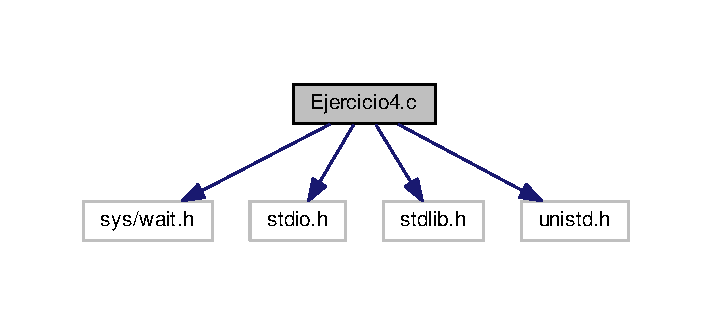
\includegraphics[width=350pt]{Ejercicio4_8c__incl}
\end{center}
\end{figure}
\subsection*{Macros}
\begin{DoxyCompactItemize}
\item 
\#define \hyperlink{Ejercicio4_8c_a9dd395f2e0046c1513c84dfcfb9e54da}{N\+U\+M\+\_\+\+H\+I\+J\+OS}~5
\end{DoxyCompactItemize}
\subsection*{Functions}
\begin{DoxyCompactItemize}
\item 
void \hyperlink{Ejercicio4_8c_a0897883a0dfdf1023f377e262cee1299}{captura} ()\hypertarget{Ejercicio4_8c_a0897883a0dfdf1023f377e262cee1299}{}\label{Ejercicio4_8c_a0897883a0dfdf1023f377e262cee1299}

\begin{DoxyCompactList}\small\item\em Funcion que ejecuta el proceso padre tras recibir la senal S\+I\+G\+U\+S\+R1. De esta forma, nos aseguramos que el proceso salga correctamente del pause() y continue su ejecucion. \end{DoxyCompactList}\item 
void \hyperlink{Ejercicio4_8c_a8dde52fc2d8703ce2fa56ebedcacee05}{terminar} ()\hypertarget{Ejercicio4_8c_a8dde52fc2d8703ce2fa56ebedcacee05}{}\label{Ejercicio4_8c_a8dde52fc2d8703ce2fa56ebedcacee05}

\begin{DoxyCompactList}\small\item\em Funcion que ejecutan los procesos hijos tras recibir la senal S\+I\+G\+U\+S\+R2, para terminar asi su ejecucion. \end{DoxyCompactList}\item 
int \hyperlink{Ejercicio4_8c_ae66f6b31b5ad750f1fe042a706a4e3d4}{main} ()
\begin{DoxyCompactList}\small\item\em El proceso padre crea un proceso hijo, que imprime 10 veces \char`\"{}\+Soy $<$\+P\+I\+D$>$ y estoy trabajando\char`\"{}, esperando un segundo entre cada vez. Una vez el proceso hijo ha impreso el texto las 10 veces, manda la señal S\+I\+G\+U\+S\+R1 al padre, que sale del pause(), y crea otro hijo, de forma que es este nuevo hijo el que manda una senal S\+I\+G\+U\+S\+R2 al hijo anterior para que este se termine a el mismo. Asi, el padre acaba creando N\+U\+M\+\_\+\+H\+I\+J\+OS procesos hijos, el mismo mata al ultimo de los hijos, y se asegura de esperar a todos. \end{DoxyCompactList}\end{DoxyCompactItemize}


\subsection{Detailed Description}
Ejercicio 4 de la Practica 2. 

\begin{DoxyAuthor}{Author}
\href{mailto:Javier.delgadod@estudiante.uam.es}{\tt Javier.\+delgadod@estudiante.\+uam.\+es} 

\href{mailto:Javier.lopezcano@estudiante.uam.es}{\tt Javier.\+lopezcano@estudiante.\+uam.\+es} 
\end{DoxyAuthor}


\subsection{Macro Definition Documentation}
\index{Ejercicio4.\+c@{Ejercicio4.\+c}!N\+U\+M\+\_\+\+H\+I\+J\+OS@{N\+U\+M\+\_\+\+H\+I\+J\+OS}}
\index{N\+U\+M\+\_\+\+H\+I\+J\+OS@{N\+U\+M\+\_\+\+H\+I\+J\+OS}!Ejercicio4.\+c@{Ejercicio4.\+c}}
\subsubsection[{\texorpdfstring{N\+U\+M\+\_\+\+H\+I\+J\+OS}{NUM_HIJOS}}]{\setlength{\rightskip}{0pt plus 5cm}\#define N\+U\+M\+\_\+\+H\+I\+J\+OS~5}\hypertarget{Ejercicio4_8c_a9dd395f2e0046c1513c84dfcfb9e54da}{}\label{Ejercicio4_8c_a9dd395f2e0046c1513c84dfcfb9e54da}
Numero de hijos que crea el proceso padre 

\subsection{Function Documentation}
\index{Ejercicio4.\+c@{Ejercicio4.\+c}!main@{main}}
\index{main@{main}!Ejercicio4.\+c@{Ejercicio4.\+c}}
\subsubsection[{\texorpdfstring{main()}{main()}}]{\setlength{\rightskip}{0pt plus 5cm}int main (
\begin{DoxyParamCaption}
\item[{void}]{}
\end{DoxyParamCaption}
)}\hypertarget{Ejercicio4_8c_ae66f6b31b5ad750f1fe042a706a4e3d4}{}\label{Ejercicio4_8c_ae66f6b31b5ad750f1fe042a706a4e3d4}


El proceso padre crea un proceso hijo, que imprime 10 veces \char`\"{}\+Soy $<$\+P\+I\+D$>$ y estoy trabajando\char`\"{}, esperando un segundo entre cada vez. Una vez el proceso hijo ha impreso el texto las 10 veces, manda la señal S\+I\+G\+U\+S\+R1 al padre, que sale del pause(), y crea otro hijo, de forma que es este nuevo hijo el que manda una senal S\+I\+G\+U\+S\+R2 al hijo anterior para que este se termine a el mismo. Asi, el padre acaba creando N\+U\+M\+\_\+\+H\+I\+J\+OS procesos hijos, el mismo mata al ultimo de los hijos, y se asegura de esperar a todos. 

\begin{DoxyReturn}{Returns}
int que determina si el programa se ha ejecutado o no con exito. 
\end{DoxyReturn}

\hypertarget{Ejercicio5_8c}{}\section{Ejercicio5.\+c File Reference}
\label{Ejercicio5_8c}\index{Ejercicio5.\+c@{Ejercicio5.\+c}}


Ejercicio 5 de la Practica 2.  


{\ttfamily \#include $<$sys/types.\+h$>$}\\*
{\ttfamily \#include $<$sys/ipc.\+h$>$}\\*
{\ttfamily \#include $<$sys/msg.\+h$>$}\\*
{\ttfamily \#include $<$stdio.\+h$>$}\\*
{\ttfamily \#include $<$string.\+h$>$}\\*
{\ttfamily \#include $<$stdlib.\+h$>$}\\*
{\ttfamily \#include $<$unistd.\+h$>$}\\*
{\ttfamily \#include $<$sys/wait.\+h$>$}\\*
Include dependency graph for Ejercicio5.\+c\+:
% FIG 0
\subsection*{Classes}
\begin{DoxyCompactItemize}
\item 
struct \hyperlink{struct__message}{\+\_\+message}
\end{DoxyCompactItemize}
\subsection*{Macros}
\begin{DoxyCompactItemize}
\item 
\#define {\bfseries F\+I\+L\+E\+K\+EY}~\char`\"{}/bin/ls\char`\"{}\hypertarget{Ejercicio5_8c_a68c15c5fb7f7c6f707903e6a46ab0557}{}\label{Ejercicio5_8c_a68c15c5fb7f7c6f707903e6a46ab0557}

\item 
\#define {\bfseries K\+EY}~33\hypertarget{Ejercicio5_8c_a8ae9d53f33f46cfcfcb9736e6351452a}{}\label{Ejercicio5_8c_a8ae9d53f33f46cfcfcb9736e6351452a}

\end{DoxyCompactItemize}
\subsection*{Typedefs}
\begin{DoxyCompactItemize}
\item 
typedef struct \hyperlink{struct__message}{\+\_\+message} {\bfseries message}\hypertarget{Ejercicio5_8c_aede0e57ab91cf2dc69d8c02488a1785c}{}\label{Ejercicio5_8c_aede0e57ab91cf2dc69d8c02488a1785c}

\end{DoxyCompactItemize}
\subsection*{Functions}
\begin{DoxyCompactItemize}
\item 
int \hyperlink{Ejercicio5_8c_a3c04138a5bfe5d72780bb7e82a18e627}{main} (int argc, char $\ast$$\ast$argv)
\begin{DoxyCompactList}\small\item\em El proceso padre crea una cola de mensajes y crea dos procesos hijo. El primero de estos realiza el proceso A que consiste en leer de un fichero y enviar a la cola de mensaje los datos del fichero en paquetes de 16 bytes. El segundo hijo se encarga del proceso B que consiste en acceder a la cola de mensajes y coger los mensajes del tipo 1 (los que ha puesto en la cola el proceso A) e ir modficando los caractere de este mensaje haciendo que cada letra se traforme en la letra siguiente, tras lo cual envia la nueva cadena de caracteres a la cola con el tipo 2. Tras crear a los hijos el proceso padre pasa a hacerse cargo del proceso C que consiste en recibir de la cola de mensajes los mensajes de tipo 2 (los que ha enviado el proceso B) y los imprime en el fichero de salida. Para indicar a cada proceso cuando debe dejar de buscar elementos en la cola de mensajes se ha introducido en el mensaje un campo flag que es un int que es 0 cuando el proceso debe seguir recibiendo mensajes, pero cuando estos se acaban se envia un mensaje con el flag 1 de modo que el proceso que lo reciba sepa que se trata del ultimo mensaje. \end{DoxyCompactList}\end{DoxyCompactItemize}
\subsection*{Variables}
\begin{DoxyCompactItemize}
\item 
int {\bfseries id}\hypertarget{Ejercicio5_8c_a7441ef0865bcb3db9b8064dd7375c1ea}{}\label{Ejercicio5_8c_a7441ef0865bcb3db9b8064dd7375c1ea}

\item 
key\+\_\+t {\bfseries key}\hypertarget{Ejercicio5_8c_ac8861193246fc34d8f29ac9d57b6791a}{}\label{Ejercicio5_8c_ac8861193246fc34d8f29ac9d57b6791a}

\end{DoxyCompactItemize}


\subsection{Detailed Description}
Ejercicio 5 de la Practica 2. 

\begin{DoxyAuthor}{Author}
\href{mailto:Javier.delgadod@estudiante.uam.es}{\tt Javier.\+delgadod@estudiante.\+uam.\+es} 

\href{mailto:Javier.lopezcano@estudiante.uam.es}{\tt Javier.\+lopezcano@estudiante.\+uam.\+es} 
\end{DoxyAuthor}


\subsection{Function Documentation}
\index{Ejercicio5.\+c@{Ejercicio5.\+c}!main@{main}}
\index{main@{main}!Ejercicio5.\+c@{Ejercicio5.\+c}}
\subsubsection[{\texorpdfstring{main(int argc, char $\ast$$\ast$argv)}{main(int argc, char **argv)}}]{\setlength{\rightskip}{0pt plus 5cm}int main (
\begin{DoxyParamCaption}
\item[{int}]{argc, }
\item[{char $\ast$$\ast$}]{argv}
\end{DoxyParamCaption}
)}\hypertarget{Ejercicio5_8c_a3c04138a5bfe5d72780bb7e82a18e627}{}\label{Ejercicio5_8c_a3c04138a5bfe5d72780bb7e82a18e627}


El proceso padre crea una cola de mensajes y crea dos procesos hijo. El primero de estos realiza el proceso A que consiste en leer de un fichero y enviar a la cola de mensaje los datos del fichero en paquetes de 16 bytes. El segundo hijo se encarga del proceso B que consiste en acceder a la cola de mensajes y coger los mensajes del tipo 1 (los que ha puesto en la cola el proceso A) e ir modficando los caractere de este mensaje haciendo que cada letra se traforme en la letra siguiente, tras lo cual envia la nueva cadena de caracteres a la cola con el tipo 2. Tras crear a los hijos el proceso padre pasa a hacerse cargo del proceso C que consiste en recibir de la cola de mensajes los mensajes de tipo 2 (los que ha enviado el proceso B) y los imprime en el fichero de salida. Para indicar a cada proceso cuando debe dejar de buscar elementos en la cola de mensajes se ha introducido en el mensaje un campo flag que es un int que es 0 cuando el proceso debe seguir recibiendo mensajes, pero cuando estos se acaban se envia un mensaje con el flag 1 de modo que el proceso que lo reciba sepa que se trata del ultimo mensaje. 


\begin{DoxyParams}{Parameters}
{\em argc} & int que indica el número de parametros de entrada. \\
\hline
{\em argv} & array de cadenas de caracteres que contiene todos los parametros de entrada, que en este caso son el nombre del ejecutable, y el nombre de los ficheros de entrada y de salida. \\
\hline
\end{DoxyParams}
\begin{DoxyReturn}{Returns}
int que determina si el programa se ha ejecutado o no con exito. 
\end{DoxyReturn}

\hypertarget{LibreriaSemaforos_8c}{}\section{Libreria\+Semaforos.\+c File Reference}
\label{LibreriaSemaforos_8c}\index{Libreria\+Semaforos.\+c@{Libreria\+Semaforos.\+c}}


Libreria de semaforos de la Practica 2.  


{\ttfamily \#include $<$stdio.\+h$>$}\\*
{\ttfamily \#include $<$sys/types.\+h$>$}\\*
{\ttfamily \#include $<$sys/ipc.\+h$>$}\\*
{\ttfamily \#include $<$sys/sem.\+h$>$}\\*
{\ttfamily \#include $<$errno.\+h$>$}\\*
{\ttfamily \#include $<$sys/shm.\+h$>$}\\*
{\ttfamily \#include $<$stdlib.\+h$>$}\\*
{\ttfamily \#include \char`\"{}Libreria\+Semaforos.\+h\char`\"{}}\\*
Include dependency graph for Libreria\+Semaforos.\+c\+:
% FIG 0
\subsection*{Classes}
\begin{DoxyCompactItemize}
\item 
union \hyperlink{unionsemun}{semun}
\end{DoxyCompactItemize}
\subsection*{Macros}
\begin{DoxyCompactItemize}
\item 
\#define {\bfseries S\+E\+M\+K\+EY}~75798\hypertarget{LibreriaSemaforos_8c_ada831b9e37399bf906c8184a888e28cd}{}\label{LibreriaSemaforos_8c_ada831b9e37399bf906c8184a888e28cd}

\item 
\#define {\bfseries N\+\_\+\+S\+E\+M\+A\+F\+O\+R\+OS}~2\hypertarget{LibreriaSemaforos_8c_a95c81905ff3d55e62fb763f407f9fab1}{}\label{LibreriaSemaforos_8c_a95c81905ff3d55e62fb763f407f9fab1}

\end{DoxyCompactItemize}
\subsection*{Functions}
\begin{DoxyCompactItemize}
\item 
int \hyperlink{LibreriaSemaforos_8c_a4af104b0ed37e6ae0289a1059bc6e990}{Inicializar\+\_\+\+Semaforo} (int semid, unsigned short $\ast$array)
\begin{DoxyCompactList}\small\item\em Función que inicializa un array de semaforos con id semid y con los valores que se pasan a traves del array de shorts. \end{DoxyCompactList}\item 
int \hyperlink{LibreriaSemaforos_8c_a731339337960a681efa435a10f12c312}{Borrar\+\_\+\+Semaforo} (int semid)
\begin{DoxyCompactList}\small\item\em Función que elimina un array de semaforos. \end{DoxyCompactList}\item 
int \hyperlink{LibreriaSemaforos_8c_a16b16dd895b5f4cbe48f1ac8977e8b35}{Crear\+\_\+\+Semaforo} (key\+\_\+t key, int size, int $\ast$semid)
\begin{DoxyCompactList}\small\item\em Funcion que crea un array de semaforos. \end{DoxyCompactList}\item 
int \hyperlink{LibreriaSemaforos_8c_a883244cd3b83c42cda23687da1b63369}{Down\+\_\+\+Semaforo} (int id, int num\+\_\+sem, int undo)
\begin{DoxyCompactList}\small\item\em Funcion que baja un semaforo. \end{DoxyCompactList}\item 
int \hyperlink{LibreriaSemaforos_8c_ab375ebfc38acbdced46e062a689d5fad}{Down\+Multiple\+\_\+\+Semaforo} (int id, int size, int undo, int $\ast$active)
\begin{DoxyCompactList}\small\item\em Funcion que baja varios semaforos de un array llamando varias veces a Down\+\_\+\+Semaforo. \end{DoxyCompactList}\item 
int \hyperlink{LibreriaSemaforos_8c_a2d5e735aecee4f493898b3d4ebab1a10}{Up\+\_\+\+Semaforo} (int id, int num\+\_\+sem, int undo)
\begin{DoxyCompactList}\small\item\em Funcion que sube un semaforo. \end{DoxyCompactList}\item 
int \hyperlink{LibreriaSemaforos_8c_a943759695f018d64a94b8a2c49308092}{Up\+Multiple\+\_\+\+Semaforo} (int id, int size, int undo, int $\ast$active)
\begin{DoxyCompactList}\small\item\em Funcion que sube varios semaforos de un array llamando varias veces a Up\+\_\+\+Semaforo. \end{DoxyCompactList}\item 
int \hyperlink{LibreriaSemaforos_8c_ac8da963855e09bf929c085486f4a3b47}{test} ()
\begin{DoxyCompactList}\small\item\em Programa que prueba el funcionamiento de la libreria. \end{DoxyCompactList}\end{DoxyCompactItemize}
\subsection*{Variables}
\begin{DoxyCompactItemize}
\item 
union \hyperlink{unionsemun}{semun} {\bfseries arg}\hypertarget{LibreriaSemaforos_8c_a7c4d098a46a7276dc49238b0590c594a}{}\label{LibreriaSemaforos_8c_a7c4d098a46a7276dc49238b0590c594a}

\end{DoxyCompactItemize}


\subsection{Detailed Description}
Libreria de semaforos de la Practica 2. 

\begin{DoxyAuthor}{Author}
\href{mailto:Javier.delgadod@estudiante.uam.es}{\tt Javier.\+delgadod@estudiante.\+uam.\+es} 

\href{mailto:Javier.lopezcano@estudiante.uam.es}{\tt Javier.\+lopezcano@estudiante.\+uam.\+es} 
\end{DoxyAuthor}


\subsection{Function Documentation}
\index{Libreria\+Semaforos.\+c@{Libreria\+Semaforos.\+c}!Borrar\+\_\+\+Semaforo@{Borrar\+\_\+\+Semaforo}}
\index{Borrar\+\_\+\+Semaforo@{Borrar\+\_\+\+Semaforo}!Libreria\+Semaforos.\+c@{Libreria\+Semaforos.\+c}}
\subsubsection[{\texorpdfstring{Borrar\+\_\+\+Semaforo(int semid)}{Borrar_Semaforo(int semid)}}]{\setlength{\rightskip}{0pt plus 5cm}int Borrar\+\_\+\+Semaforo (
\begin{DoxyParamCaption}
\item[{int}]{semid}
\end{DoxyParamCaption}
)}\hypertarget{LibreriaSemaforos_8c_a731339337960a681efa435a10f12c312}{}\label{LibreriaSemaforos_8c_a731339337960a681efa435a10f12c312}


Función que elimina un array de semaforos. 


\begin{DoxyParams}{Parameters}
{\em semid} & Int que es el id del array de semáforos. \\
\hline
\end{DoxyParams}
\begin{DoxyReturn}{Returns}
int que determina si la funcion se ha ejecutado o no con exito. 
\end{DoxyReturn}
\index{Libreria\+Semaforos.\+c@{Libreria\+Semaforos.\+c}!Crear\+\_\+\+Semaforo@{Crear\+\_\+\+Semaforo}}
\index{Crear\+\_\+\+Semaforo@{Crear\+\_\+\+Semaforo}!Libreria\+Semaforos.\+c@{Libreria\+Semaforos.\+c}}
\subsubsection[{\texorpdfstring{Crear\+\_\+\+Semaforo(key\+\_\+t key, int size, int $\ast$semid)}{Crear_Semaforo(key_t key, int size, int *semid)}}]{\setlength{\rightskip}{0pt plus 5cm}int Crear\+\_\+\+Semaforo (
\begin{DoxyParamCaption}
\item[{key\+\_\+t}]{key, }
\item[{int}]{size, }
\item[{int $\ast$}]{semid}
\end{DoxyParamCaption}
)}\hypertarget{LibreriaSemaforos_8c_a16b16dd895b5f4cbe48f1ac8977e8b35}{}\label{LibreriaSemaforos_8c_a16b16dd895b5f4cbe48f1ac8977e8b35}


Funcion que crea un array de semaforos. 


\begin{DoxyParams}{Parameters}
{\em key} & Identificador de I\+PC. \\
\hline
{\em size} & Tamano del array de semaforos que se quiere crear. \\
\hline
{\em semid} & Int que es el id del array de semáforos. \\
\hline
\end{DoxyParams}
\begin{DoxyReturn}{Returns}
int que determina si la funcion se ha ejecutado o no con exito. 
\end{DoxyReturn}
\index{Libreria\+Semaforos.\+c@{Libreria\+Semaforos.\+c}!Down\+\_\+\+Semaforo@{Down\+\_\+\+Semaforo}}
\index{Down\+\_\+\+Semaforo@{Down\+\_\+\+Semaforo}!Libreria\+Semaforos.\+c@{Libreria\+Semaforos.\+c}}
\subsubsection[{\texorpdfstring{Down\+\_\+\+Semaforo(int id, int num\+\_\+sem, int undo)}{Down_Semaforo(int id, int num_sem, int undo)}}]{\setlength{\rightskip}{0pt plus 5cm}int Down\+\_\+\+Semaforo (
\begin{DoxyParamCaption}
\item[{int}]{id, }
\item[{int}]{num\+\_\+sem, }
\item[{int}]{undo}
\end{DoxyParamCaption}
)}\hypertarget{LibreriaSemaforos_8c_a883244cd3b83c42cda23687da1b63369}{}\label{LibreriaSemaforos_8c_a883244cd3b83c42cda23687da1b63369}


Funcion que baja un semaforo. 


\begin{DoxyParams}{Parameters}
{\em id} & Int con el id del array de semaforos. \\
\hline
{\em num\+\_\+sem} & Int con el indice del semaforo que se quiere bajar. \\
\hline
{\em undo} & Int que es la bandera que hay que usar en la estructura sem\+\_\+oper. \\
\hline
\end{DoxyParams}
\begin{DoxyReturn}{Returns}
int que determina si la funcion se ha ejecutado o no con exito. 
\end{DoxyReturn}
\index{Libreria\+Semaforos.\+c@{Libreria\+Semaforos.\+c}!Down\+Multiple\+\_\+\+Semaforo@{Down\+Multiple\+\_\+\+Semaforo}}
\index{Down\+Multiple\+\_\+\+Semaforo@{Down\+Multiple\+\_\+\+Semaforo}!Libreria\+Semaforos.\+c@{Libreria\+Semaforos.\+c}}
\subsubsection[{\texorpdfstring{Down\+Multiple\+\_\+\+Semaforo(int id, int size, int undo, int $\ast$active)}{DownMultiple_Semaforo(int id, int size, int undo, int *active)}}]{\setlength{\rightskip}{0pt plus 5cm}int Down\+Multiple\+\_\+\+Semaforo (
\begin{DoxyParamCaption}
\item[{int}]{id, }
\item[{int}]{size, }
\item[{int}]{undo, }
\item[{int $\ast$}]{active}
\end{DoxyParamCaption}
)}\hypertarget{LibreriaSemaforos_8c_ab375ebfc38acbdced46e062a689d5fad}{}\label{LibreriaSemaforos_8c_ab375ebfc38acbdced46e062a689d5fad}


Funcion que baja varios semaforos de un array llamando varias veces a Down\+\_\+\+Semaforo. 


\begin{DoxyParams}{Parameters}
{\em id} & Int con el id del array de semaforos. \\
\hline
{\em size} & Int con el tamano del array de semaforos. \\
\hline
{\em undo} & Int que es la bandera que hay que usar en la estructura sem\+\_\+oper. \\
\hline
{\em active} & Array de int con los indices de los semaforos que se quiere bajar. \\
\hline
\end{DoxyParams}
\begin{DoxyReturn}{Returns}
int que determina si la funcion se ha ejecutado o no con exito. 
\end{DoxyReturn}
\index{Libreria\+Semaforos.\+c@{Libreria\+Semaforos.\+c}!Inicializar\+\_\+\+Semaforo@{Inicializar\+\_\+\+Semaforo}}
\index{Inicializar\+\_\+\+Semaforo@{Inicializar\+\_\+\+Semaforo}!Libreria\+Semaforos.\+c@{Libreria\+Semaforos.\+c}}
\subsubsection[{\texorpdfstring{Inicializar\+\_\+\+Semaforo(int semid, unsigned short $\ast$array)}{Inicializar_Semaforo(int semid, unsigned short *array)}}]{\setlength{\rightskip}{0pt plus 5cm}int Inicializar\+\_\+\+Semaforo (
\begin{DoxyParamCaption}
\item[{int}]{semid, }
\item[{unsigned short $\ast$}]{array}
\end{DoxyParamCaption}
)}\hypertarget{LibreriaSemaforos_8c_a4af104b0ed37e6ae0289a1059bc6e990}{}\label{LibreriaSemaforos_8c_a4af104b0ed37e6ae0289a1059bc6e990}


Función que inicializa un array de semaforos con id semid y con los valores que se pasan a traves del array de shorts. 


\begin{DoxyParams}{Parameters}
{\em semid} & Int que es el id del array de semaforos. \\
\hline
{\em array} & Array de shorts con la informacion para inicializar los semaforos. \\
\hline
\end{DoxyParams}
\begin{DoxyReturn}{Returns}
int que determina si la funcion se ha ejecutado o no con exito. 
\end{DoxyReturn}
\index{Libreria\+Semaforos.\+c@{Libreria\+Semaforos.\+c}!test@{test}}
\index{test@{test}!Libreria\+Semaforos.\+c@{Libreria\+Semaforos.\+c}}
\subsubsection[{\texorpdfstring{test()}{test()}}]{\setlength{\rightskip}{0pt plus 5cm}int test (
\begin{DoxyParamCaption}
{}
\end{DoxyParamCaption}
)}\hypertarget{LibreriaSemaforos_8c_ac8da963855e09bf929c085486f4a3b47}{}\label{LibreriaSemaforos_8c_ac8da963855e09bf929c085486f4a3b47}


Programa que prueba el funcionamiento de la libreria. 

\begin{DoxyReturn}{Returns}
int que determina si el programa se ha ejecutado o no con exito. 
\end{DoxyReturn}
\index{Libreria\+Semaforos.\+c@{Libreria\+Semaforos.\+c}!Up\+\_\+\+Semaforo@{Up\+\_\+\+Semaforo}}
\index{Up\+\_\+\+Semaforo@{Up\+\_\+\+Semaforo}!Libreria\+Semaforos.\+c@{Libreria\+Semaforos.\+c}}
\subsubsection[{\texorpdfstring{Up\+\_\+\+Semaforo(int id, int num\+\_\+sem, int undo)}{Up_Semaforo(int id, int num_sem, int undo)}}]{\setlength{\rightskip}{0pt plus 5cm}int Up\+\_\+\+Semaforo (
\begin{DoxyParamCaption}
\item[{int}]{id, }
\item[{int}]{num\+\_\+sem, }
\item[{int}]{undo}
\end{DoxyParamCaption}
)}\hypertarget{LibreriaSemaforos_8c_a2d5e735aecee4f493898b3d4ebab1a10}{}\label{LibreriaSemaforos_8c_a2d5e735aecee4f493898b3d4ebab1a10}


Funcion que sube un semaforo. 


\begin{DoxyParams}{Parameters}
{\em id} & Int con el id del array de semaforos. \\
\hline
{\em num\+\_\+sem} & Int con el indice del semaforo que se quiere subir. \\
\hline
{\em undo} & Int que es la bandera que hay que usar en la estructura sem\+\_\+oper. \\
\hline
\end{DoxyParams}
\begin{DoxyReturn}{Returns}
int que determina si la funcion se ha ejecutado o no con exito. 
\end{DoxyReturn}
\index{Libreria\+Semaforos.\+c@{Libreria\+Semaforos.\+c}!Up\+Multiple\+\_\+\+Semaforo@{Up\+Multiple\+\_\+\+Semaforo}}
\index{Up\+Multiple\+\_\+\+Semaforo@{Up\+Multiple\+\_\+\+Semaforo}!Libreria\+Semaforos.\+c@{Libreria\+Semaforos.\+c}}
\subsubsection[{\texorpdfstring{Up\+Multiple\+\_\+\+Semaforo(int id, int size, int undo, int $\ast$active)}{UpMultiple_Semaforo(int id, int size, int undo, int *active)}}]{\setlength{\rightskip}{0pt plus 5cm}int Up\+Multiple\+\_\+\+Semaforo (
\begin{DoxyParamCaption}
\item[{int}]{id, }
\item[{int}]{size, }
\item[{int}]{undo, }
\item[{int $\ast$}]{active}
\end{DoxyParamCaption}
)}\hypertarget{LibreriaSemaforos_8c_a943759695f018d64a94b8a2c49308092}{}\label{LibreriaSemaforos_8c_a943759695f018d64a94b8a2c49308092}


Funcion que sube varios semaforos de un array llamando varias veces a Up\+\_\+\+Semaforo. 


\begin{DoxyParams}{Parameters}
{\em id} & Int con el id del array de semaforos. \\
\hline
{\em size} & Int con el tamano del array de semaforos. \\
\hline
{\em undo} & Int que es la bandera que hay que usar en la estructura sem\+\_\+oper. \\
\hline
{\em active} & Array de int con los indices de los semaforos que se quiere subir. \\
\hline
\end{DoxyParams}
\begin{DoxyReturn}{Returns}
int que determina si la funcion se ha ejecutado o no con exito. 
\end{DoxyReturn}

\hypertarget{LibreriaSemaforos_8h}{}\section{Libreria\+Semaforos.\+h File Reference}
\label{LibreriaSemaforos_8h}\index{Libreria\+Semaforos.\+h@{Libreria\+Semaforos.\+h}}


Libreria de semaforos de la Practica 2.  


{\ttfamily \#include $<$sys/sem.\+h$>$}\\*
Include dependency graph for Libreria\+Semaforos.\+h\+:
% FIG 0
This graph shows which files directly or indirectly include this file\+:
% FIG 1
\subsection*{Macros}
\begin{DoxyCompactItemize}
\item 
\#define {\bfseries E\+R\+R\+OR}~-\/1\hypertarget{LibreriaSemaforos_8h_a8fe83ac76edc595f6b98cd4a4127aed5}{}\label{LibreriaSemaforos_8h_a8fe83ac76edc595f6b98cd4a4127aed5}

\item 
\#define {\bfseries OK}~0\hypertarget{LibreriaSemaforos_8h_aba51915c87d64af47fb1cc59348961c9}{}\label{LibreriaSemaforos_8h_aba51915c87d64af47fb1cc59348961c9}

\item 
\#define {\bfseries C\+R\+E\+A\+DO}~1\hypertarget{LibreriaSemaforos_8h_a00182e3826731997fd4a69a493fac3dd}{}\label{LibreriaSemaforos_8h_a00182e3826731997fd4a69a493fac3dd}

\end{DoxyCompactItemize}
\subsection*{Functions}
\begin{DoxyCompactItemize}
\item 
int \hyperlink{LibreriaSemaforos_8h_a4af104b0ed37e6ae0289a1059bc6e990}{Inicializar\+\_\+\+Semaforo} (int semid, unsigned short $\ast$array)
\begin{DoxyCompactList}\small\item\em Función que inicializa un array de semaforos con id semid y con los valores que se pasan a traves del array de shorts. \end{DoxyCompactList}\item 
int \hyperlink{LibreriaSemaforos_8h_a731339337960a681efa435a10f12c312}{Borrar\+\_\+\+Semaforo} (int semid)
\begin{DoxyCompactList}\small\item\em Función que elimina un array de semaforos. \end{DoxyCompactList}\item 
int \hyperlink{LibreriaSemaforos_8h_a16b16dd895b5f4cbe48f1ac8977e8b35}{Crear\+\_\+\+Semaforo} (key\+\_\+t key, int size, int $\ast$semid)
\begin{DoxyCompactList}\small\item\em Funcion que crea un array de semaforos. \end{DoxyCompactList}\item 
int \hyperlink{LibreriaSemaforos_8h_a883244cd3b83c42cda23687da1b63369}{Down\+\_\+\+Semaforo} (int id, int num\+\_\+sem, int undo)
\begin{DoxyCompactList}\small\item\em Funcion que baja un semaforo. \end{DoxyCompactList}\item 
int \hyperlink{LibreriaSemaforos_8h_ab375ebfc38acbdced46e062a689d5fad}{Down\+Multiple\+\_\+\+Semaforo} (int id, int size, int undo, int $\ast$active)
\begin{DoxyCompactList}\small\item\em Funcion que baja varios semaforos de un array llamando varias veces a Down\+\_\+\+Semaforo. \end{DoxyCompactList}\item 
int \hyperlink{LibreriaSemaforos_8h_a2d5e735aecee4f493898b3d4ebab1a10}{Up\+\_\+\+Semaforo} (int id, int num\+\_\+sem, int undo)
\begin{DoxyCompactList}\small\item\em Funcion que sube un semaforo. \end{DoxyCompactList}\item 
int \hyperlink{LibreriaSemaforos_8h_a943759695f018d64a94b8a2c49308092}{Up\+Multiple\+\_\+\+Semaforo} (int id, int size, int undo, int $\ast$active)
\begin{DoxyCompactList}\small\item\em Funcion que sube varios semaforos de un array llamando varias veces a Up\+\_\+\+Semaforo. \end{DoxyCompactList}\end{DoxyCompactItemize}


\subsection{Detailed Description}
Libreria de semaforos de la Practica 2. 

\begin{DoxyAuthor}{Author}
\href{mailto:Javier.delgadod@estudiante.uam.es}{\tt Javier.\+delgadod@estudiante.\+uam.\+es} 

\href{mailto:Javier.lopezcano@estudiante.uam.es}{\tt Javier.\+lopezcano@estudiante.\+uam.\+es} 
\end{DoxyAuthor}


\subsection{Function Documentation}
\index{Libreria\+Semaforos.\+h@{Libreria\+Semaforos.\+h}!Borrar\+\_\+\+Semaforo@{Borrar\+\_\+\+Semaforo}}
\index{Borrar\+\_\+\+Semaforo@{Borrar\+\_\+\+Semaforo}!Libreria\+Semaforos.\+h@{Libreria\+Semaforos.\+h}}
\subsubsection[{\texorpdfstring{Borrar\+\_\+\+Semaforo(int semid)}{Borrar_Semaforo(int semid)}}]{\setlength{\rightskip}{0pt plus 5cm}int Borrar\+\_\+\+Semaforo (
\begin{DoxyParamCaption}
\item[{int}]{semid}
\end{DoxyParamCaption}
)}\hypertarget{LibreriaSemaforos_8h_a731339337960a681efa435a10f12c312}{}\label{LibreriaSemaforos_8h_a731339337960a681efa435a10f12c312}


Función que elimina un array de semaforos. 


\begin{DoxyParams}{Parameters}
{\em semid} & Int que es el id del array de semáforos. \\
\hline
\end{DoxyParams}
\begin{DoxyReturn}{Returns}
int que determina si la funcion se ha ejecutado o no con exito. 
\end{DoxyReturn}
\index{Libreria\+Semaforos.\+h@{Libreria\+Semaforos.\+h}!Crear\+\_\+\+Semaforo@{Crear\+\_\+\+Semaforo}}
\index{Crear\+\_\+\+Semaforo@{Crear\+\_\+\+Semaforo}!Libreria\+Semaforos.\+h@{Libreria\+Semaforos.\+h}}
\subsubsection[{\texorpdfstring{Crear\+\_\+\+Semaforo(key\+\_\+t key, int size, int $\ast$semid)}{Crear_Semaforo(key_t key, int size, int *semid)}}]{\setlength{\rightskip}{0pt plus 5cm}int Crear\+\_\+\+Semaforo (
\begin{DoxyParamCaption}
\item[{key\+\_\+t}]{key, }
\item[{int}]{size, }
\item[{int $\ast$}]{semid}
\end{DoxyParamCaption}
)}\hypertarget{LibreriaSemaforos_8h_a16b16dd895b5f4cbe48f1ac8977e8b35}{}\label{LibreriaSemaforos_8h_a16b16dd895b5f4cbe48f1ac8977e8b35}


Funcion que crea un array de semaforos. 


\begin{DoxyParams}{Parameters}
{\em key} & Identificador de I\+PC. \\
\hline
{\em size} & Tamano del array de semaforos que se quiere crear. \\
\hline
{\em semid} & Int que es el id del array de semáforos. \\
\hline
\end{DoxyParams}
\begin{DoxyReturn}{Returns}
int que determina si la funcion se ha ejecutado o no con exito. 
\end{DoxyReturn}
\index{Libreria\+Semaforos.\+h@{Libreria\+Semaforos.\+h}!Down\+\_\+\+Semaforo@{Down\+\_\+\+Semaforo}}
\index{Down\+\_\+\+Semaforo@{Down\+\_\+\+Semaforo}!Libreria\+Semaforos.\+h@{Libreria\+Semaforos.\+h}}
\subsubsection[{\texorpdfstring{Down\+\_\+\+Semaforo(int id, int num\+\_\+sem, int undo)}{Down_Semaforo(int id, int num_sem, int undo)}}]{\setlength{\rightskip}{0pt plus 5cm}int Down\+\_\+\+Semaforo (
\begin{DoxyParamCaption}
\item[{int}]{id, }
\item[{int}]{num\+\_\+sem, }
\item[{int}]{undo}
\end{DoxyParamCaption}
)}\hypertarget{LibreriaSemaforos_8h_a883244cd3b83c42cda23687da1b63369}{}\label{LibreriaSemaforos_8h_a883244cd3b83c42cda23687da1b63369}


Funcion que baja un semaforo. 


\begin{DoxyParams}{Parameters}
{\em id} & Int con el id del array de semaforos. \\
\hline
{\em num\+\_\+sem} & Int con el indice del semaforo que se quiere bajar. \\
\hline
{\em undo} & Int que es la bandera que hay que usar en la estructura sem\+\_\+oper. \\
\hline
\end{DoxyParams}
\begin{DoxyReturn}{Returns}
int que determina si la funcion se ha ejecutado o no con exito. 
\end{DoxyReturn}
\index{Libreria\+Semaforos.\+h@{Libreria\+Semaforos.\+h}!Down\+Multiple\+\_\+\+Semaforo@{Down\+Multiple\+\_\+\+Semaforo}}
\index{Down\+Multiple\+\_\+\+Semaforo@{Down\+Multiple\+\_\+\+Semaforo}!Libreria\+Semaforos.\+h@{Libreria\+Semaforos.\+h}}
\subsubsection[{\texorpdfstring{Down\+Multiple\+\_\+\+Semaforo(int id, int size, int undo, int $\ast$active)}{DownMultiple_Semaforo(int id, int size, int undo, int *active)}}]{\setlength{\rightskip}{0pt plus 5cm}int Down\+Multiple\+\_\+\+Semaforo (
\begin{DoxyParamCaption}
\item[{int}]{id, }
\item[{int}]{size, }
\item[{int}]{undo, }
\item[{int $\ast$}]{active}
\end{DoxyParamCaption}
)}\hypertarget{LibreriaSemaforos_8h_ab375ebfc38acbdced46e062a689d5fad}{}\label{LibreriaSemaforos_8h_ab375ebfc38acbdced46e062a689d5fad}


Funcion que baja varios semaforos de un array llamando varias veces a Down\+\_\+\+Semaforo. 


\begin{DoxyParams}{Parameters}
{\em id} & Int con el id del array de semaforos. \\
\hline
{\em size} & Int con el tamano del array de semaforos. \\
\hline
{\em undo} & Int que es la bandera que hay que usar en la estructura sem\+\_\+oper. \\
\hline
{\em active} & Array de int con los indices de los semaforos que se quiere bajar. \\
\hline
\end{DoxyParams}
\begin{DoxyReturn}{Returns}
int que determina si la funcion se ha ejecutado o no con exito. 
\end{DoxyReturn}
\index{Libreria\+Semaforos.\+h@{Libreria\+Semaforos.\+h}!Inicializar\+\_\+\+Semaforo@{Inicializar\+\_\+\+Semaforo}}
\index{Inicializar\+\_\+\+Semaforo@{Inicializar\+\_\+\+Semaforo}!Libreria\+Semaforos.\+h@{Libreria\+Semaforos.\+h}}
\subsubsection[{\texorpdfstring{Inicializar\+\_\+\+Semaforo(int semid, unsigned short $\ast$array)}{Inicializar_Semaforo(int semid, unsigned short *array)}}]{\setlength{\rightskip}{0pt plus 5cm}int Inicializar\+\_\+\+Semaforo (
\begin{DoxyParamCaption}
\item[{int}]{semid, }
\item[{unsigned short $\ast$}]{array}
\end{DoxyParamCaption}
)}\hypertarget{LibreriaSemaforos_8h_a4af104b0ed37e6ae0289a1059bc6e990}{}\label{LibreriaSemaforos_8h_a4af104b0ed37e6ae0289a1059bc6e990}


Función que inicializa un array de semaforos con id semid y con los valores que se pasan a traves del array de shorts. 


\begin{DoxyParams}{Parameters}
{\em semid} & Int que es el id del array de semaforos. \\
\hline
{\em array} & Array de shorts con la informacion para inicializar los semaforos. \\
\hline
\end{DoxyParams}
\begin{DoxyReturn}{Returns}
int que determina si la funcion se ha ejecutado o no con exito. 
\end{DoxyReturn}
\index{Libreria\+Semaforos.\+h@{Libreria\+Semaforos.\+h}!Up\+\_\+\+Semaforo@{Up\+\_\+\+Semaforo}}
\index{Up\+\_\+\+Semaforo@{Up\+\_\+\+Semaforo}!Libreria\+Semaforos.\+h@{Libreria\+Semaforos.\+h}}
\subsubsection[{\texorpdfstring{Up\+\_\+\+Semaforo(int id, int num\+\_\+sem, int undo)}{Up_Semaforo(int id, int num_sem, int undo)}}]{\setlength{\rightskip}{0pt plus 5cm}int Up\+\_\+\+Semaforo (
\begin{DoxyParamCaption}
\item[{int}]{id, }
\item[{int}]{num\+\_\+sem, }
\item[{int}]{undo}
\end{DoxyParamCaption}
)}\hypertarget{LibreriaSemaforos_8h_a2d5e735aecee4f493898b3d4ebab1a10}{}\label{LibreriaSemaforos_8h_a2d5e735aecee4f493898b3d4ebab1a10}


Funcion que sube un semaforo. 


\begin{DoxyParams}{Parameters}
{\em id} & Int con el id del array de semaforos. \\
\hline
{\em num\+\_\+sem} & Int con el indice del semaforo que se quiere subir. \\
\hline
{\em undo} & Int que es la bandera que hay que usar en la estructura sem\+\_\+oper. \\
\hline
\end{DoxyParams}
\begin{DoxyReturn}{Returns}
int que determina si la funcion se ha ejecutado o no con exito. 
\end{DoxyReturn}
\index{Libreria\+Semaforos.\+h@{Libreria\+Semaforos.\+h}!Up\+Multiple\+\_\+\+Semaforo@{Up\+Multiple\+\_\+\+Semaforo}}
\index{Up\+Multiple\+\_\+\+Semaforo@{Up\+Multiple\+\_\+\+Semaforo}!Libreria\+Semaforos.\+h@{Libreria\+Semaforos.\+h}}
\subsubsection[{\texorpdfstring{Up\+Multiple\+\_\+\+Semaforo(int id, int size, int undo, int $\ast$active)}{UpMultiple_Semaforo(int id, int size, int undo, int *active)}}]{\setlength{\rightskip}{0pt plus 5cm}int Up\+Multiple\+\_\+\+Semaforo (
\begin{DoxyParamCaption}
\item[{int}]{id, }
\item[{int}]{size, }
\item[{int}]{undo, }
\item[{int $\ast$}]{active}
\end{DoxyParamCaption}
)}\hypertarget{LibreriaSemaforos_8h_a943759695f018d64a94b8a2c49308092}{}\label{LibreriaSemaforos_8h_a943759695f018d64a94b8a2c49308092}


Funcion que sube varios semaforos de un array llamando varias veces a Up\+\_\+\+Semaforo. 


\begin{DoxyParams}{Parameters}
{\em id} & Int con el id del array de semaforos. \\
\hline
{\em size} & Int con el tamano del array de semaforos. \\
\hline
{\em undo} & Int que es la bandera que hay que usar en la estructura sem\+\_\+oper. \\
\hline
{\em active} & Array de int con los indices de los semaforos que se quiere subir. \\
\hline
\end{DoxyParams}
\begin{DoxyReturn}{Returns}
int que determina si la funcion se ha ejecutado o no con exito. 
\end{DoxyReturn}

%--- End generated contents ---

% Index
\backmatter
\newpage
\phantomsection
\clearemptydoublepage
\addcontentsline{toc}{chapter}{Index}
\printindex

\end{document}
